\chapter{Methodology}

\section{Project Management and Research}
The first project meeting began in the final week of September, briefly after the project requirements had been defined and outlined. An early start was agreed to be something that would greatly benefit the overall development of the project and it was concluded that an idea should be finalized as soon as possible to allow for necessary pre-development research.

\paragraph{}
This section will further explore the aforementioned pre-development process, the influence of the supervisory meetings on this stage and the overall methodical conclusion and it's influence on the initial project direction.

\subsection{Brainstorming and Initial Supervisory Meeting}
In the weeks before development began, after the project idea had been finalized, technologies, concepts and potential inclusions were explored and discussed between the team members. A brainstorming phase was conducted on what to incorporate into the project.

\subsubsection{Brainstorming}
The team members met prior to the initial supervisory meeting to discuss potential avenues of exploration during the development phase. To produce effective ideas, questions had to be asked relating to the ultimate goals and objectives of the project, these included:

\begin{itemize}
    \item\textit{\textbf{What research areas should be prioritized before the development phase is initialized?}}
    \item\textit{\textbf{What type of Methodology would best fit our approach?}}
    \item\textit{\textbf{What benefits would different methodologies have when compared to others?}}
\end{itemize}

\subsubsection{Initial Supervisory Meeting}
During the initial supervisory meeting following the project decision, potential research and developmental approaches were discussed and the team were advised to spend the next week heavily considering the nature of how the project will be implemented. All parties agreed external considerations and feedback were important for the nature of the project considering students will be the end users. 

\paragraph{}
Following the supervisory meeting the team decided to research avenues for allowing other students a platform to contribute suggestions and ideas. This was felt to be an important inclusion since, while the team consists of students, it would be highly valuable and beneficial for the health and development of the project employ the ideas and feedback of multiple potential end users.

\subsection{Research Methodology Consideration}
The team felt there was a clear direction to take when it came to gathering opinions and information from fellow college students, meaning a comparative analysis of methodical approach wasn't necessary. Face to face discussions with students along with a brief survey on student accommodation and related accommodation applications would be necessary mediums for gathering information.

\subsection{Development Methodology Consideration}
There were numerous possible methodologies to consider, namely Waterfall, Rapid Application Development and Agile to name a few. Following discussions internally between the team members and talks with supervisors, the list of potential methodologies were shortlisted to both \textbf{Waterfall} and \textbf{Agile}.

\section{Gathering Information}
Following the decision to employ both surveying and face to face methods for gathering information, a short online survey was constructed with the following questions:

\begin{enumerate}
    \item\textit{\textbf{How many students do you know that are currently renting accommodation local to the College?}}
    \item\textit{\textbf{Out of those students, how many do you know of that are unhappy with their current living situation?}}
    \item\textit{\textbf{What applications are you aware of that you (or those you know) would use to find accommodation local to your college?}}
    \item\textit{\textbf{If an application was developed specifically to help students in Galway find local accommodation, would you or students you know be interested?}}
    \item\textit{\textbf{What features would you like to see in the application?}}
\end{enumerate}

The team felt the choice to have as few questions as possible would be a valuable decision in terms of encouraging more students to partake. The goal was to avoid students feeling intimidated by an otherwise overwhelming barrage of questions.

\subsubsection{Distributing the Survey}
The survey was sent to various friends and students within the course. Recipients of the survey were encouraged to distribute the survey to friends of theirs who were also students. Responses were accepted for three weeks following the distribution. 

\subsection{Survey Results}
Following the closure of responses the team were very happy with the higher than expected overall response to the survey \cite{SURVEY}. Twenty-one students participated in the survey altogether, the great response rate was likely due to the simplicity and briefness of the survey. 

\paragraph{}
This subsection will act as a brief analysis of the responses given for the major questions in the survey.

\paragraph{}
Initially the recipients were asked how many students were they aware of that were renting locally to the college and based on that answer, were prompted to answer how many of those same students were unhappy with their current living situation.

\subsubsection{Student Accommodative Unhappiness}
This part of the survey was important in gauging the rough amount of students that are unhappy with their current living situation. Based on this result, it would be possible to see if the necessity of an accommodation application targeted at students would even be warranted.

\begin{figure}[H]
	\caption{Student Unhappiness}
	\label{image:surveyHappy}
	\centering
	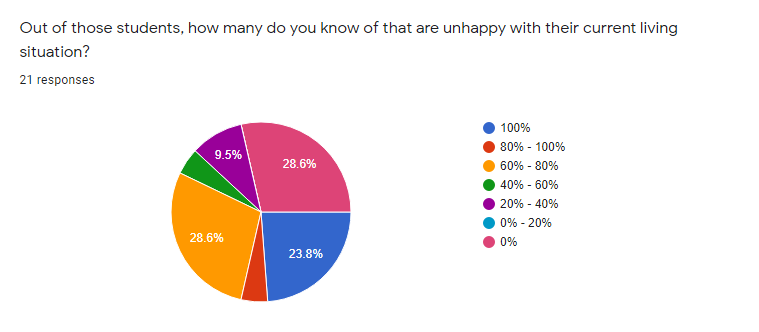
\includegraphics[width=1\textwidth]{images/survey_happy.png}
\end{figure}	

\paragraph{}
Following the closure of the survey, it can be seen from \textit{Figure.\ref{image:surveyHappy}} that just over a quarter of students are happy with their current living situation, a definitive result. Based on this response, it can be taken as a given that there is definitely a gap for a student-specific accommodation related product. Looking at the result, it can be wise to assume there isn't a similar application that is considered viable currently, and if there is it isn't effective.

\subsubsection{Student Interest}
Students were asked about their interest in a student specific accommodation application, this question was included to remove any ambiguity from the previous question if there happened to be any. 

\begin{figure}[H]
	\caption{Student Interest}
	\label{image:surveyInterest}
	\centering
	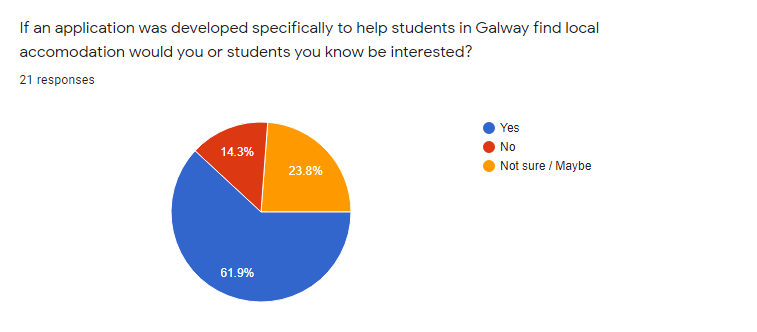
\includegraphics[width=1\textwidth]{images/survey_interest.png}
\end{figure}

\paragraph{}
Following the overwhelming positive response illustrated in \textit{Figure.\ref{image:surveyHappy}}, the results displayed in \textit{Figure.\ref{image:surveyInterest}} only confirmed what was already known, that there is definitely a gap for a product of this nature.

\subsubsection{Similar Applications}
In order to provide the team with an idea of what similar in nature applications are currently available to students, survey recipients were asked to list some applications they feel themselves or others they know would use when searching for accommodation local to their educational institute in Galway.
\begin{table}[H]
\centering
\begin{tabular}{ |p{3cm}||p{3cm}| }

 \hline
 \multicolumn{2}{|c|}{Application Occurrence} \\
 \hline
 Application & Frequency \\
 \hline
 Adverts   & 10    \\
 Daft &   6    \\
 Done Deal & 5 \\
 AirBnB    & 5 \\
 Facebook &  4  \\
 MyHome & 2 \\
 Don't Know & 3  \\
 \hline
 
\end{tabular}
\caption{Frequency of Application Occurrence}
\label{table:1}
\end{table}

\paragraph{}
Following the analysis of the results illustrated in \textit{Table.\ref{table:1}}, it became clear there wasn't an absolute front runner that all recipients would be able to name on the spot. The results were scattered, with Adverts being the most known related application. The most known application in this field being one that doesn't actually specialize in finding accommodation speaks volumes about the lack of relevant student services of this nature.

\paragraph{}
This feedback would also prove useful in the sense that the listed applications could be analysed during the development process. Key strengths of the applications could be brought on board while weaknesses and unnecessary features excluded, allowing for a more specialized student experience.

\subsubsection{Application Functionality}
Finally, recipients were asked about the features they felt would be necessary in an application of this nature. This was asked mainly to gauge the main application features that end users felt would take priority over others.

\begin{figure}[H]
	\caption{Application Feature Priority}
	\label{image:surveyInterest}
	\centering
	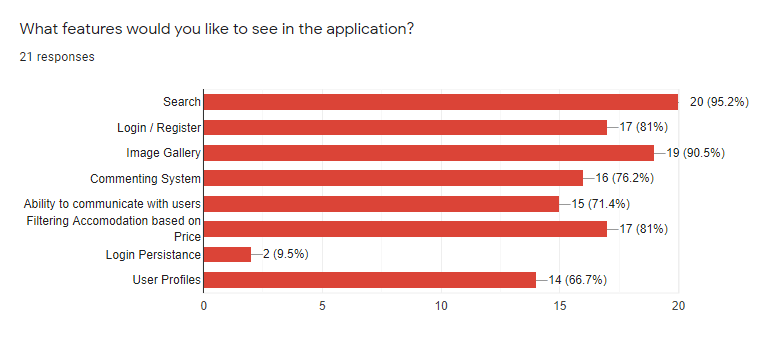
\includegraphics[width=1\textwidth]{images/survey_features.png}
\end{figure}

\paragraph{}
This response turned out to be highly valuable to the development phase of the project. The team could see first-hand the key features end users felt to be a necessity to an application of this nature. During the development phase this chart was highly referenced by the team when deciding the order of features to implement.

\subsection{Face to Face Interviews}
Following the overwhelmingly positive response of the survey, the team felt personal interviews with students would not be necessary and chose to occupy their time with working on key features mentioned by recipients of the survey.

\paragraph{}
That isn't to say students weren't consulted during the development of the project. Over the course of development students would periodically be asked their opinion on a new feature or to test a piece of functionality. This was felt to be an important process in ensuring the project remained healthy during the development phase.

\subsection{Conclusion}
The team felt very positive following the valuable feedback provided by fellow students. The need for an application of this nature was confirmed by the participants and applications that are considered similar in nature by potential end-users were provided, allowing the comparison and analysis of strengths and weaknesses of these applications, helping the team to build a platform combining the strengths and key features of similar natured applications.

\paragraph{}
Without the input, the development of the application may have gone off course, features may have been implemented that wouldn't have been considered a high priority or functionality may have been added that may make sense to the developers but end users may struggle to get a grasp of.

\section{Determining the Development Methodology}
Following the decision to shortlist both Waterfall and Agile, research began on which route would be best to take when considering the scope and overall goals of the project and comparisons between the two were drawn. A brief high-level overview of both methodologies will be included followed by comparisons and a practical analysis of each methodology in relation to the project.

\subsection{Waterfall}
Like most traditional software development models and methodologies, the Waterfall model is based on a series of phases or steps, illustrated in \textit{Figure 2.1}. Waterfall allows progress to be easily measured, the complete scope of the project is known in advance which can be preferred based on the project being undertaken. Since the overall design is finished early in the development cycle, the Waterfall approach is especially effective in projects where various software components need to be designed in parallel \cite{WATERFALL_SURVEY} 

\begin{figure}[H]
	\caption{Waterfall Model Cycle}
	\label{image:waterfall}
	\centering
	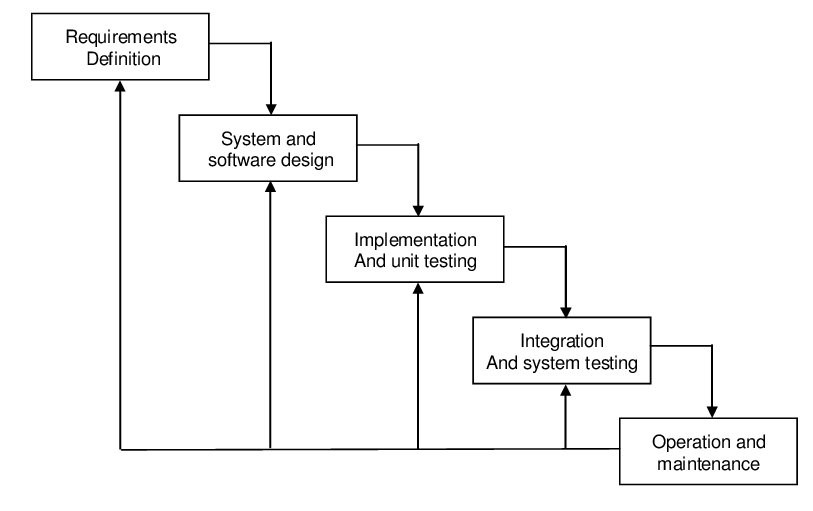
\includegraphics[width=0.9\textwidth]{images/waterfall.png}
\end{figure}	

The Waterfall model is arguably the most well known development model, which is likely attributed to how long the model has been around, not to mention it's overall simplicity. Waterfall being an easily understood model naturally means it isn't difficult to manage which is mainly attributed to it's strict requirement definitions that ensures requirements are clearly defined, well received and understood \cite{WATERFALL}. Each phase is processed and undertaken uniformly, meaning phases are completed sequentially and don't overlap \cite{WATERFALL_REVIEW}.

\subsection{Agile}
Initially described in the Manifesto for Agile Software Development, Agile is a an array of principles and methods for project management \cite{AGILE_MANIFESTO}. It is characterized by an iterate approach that allows software to be delivered to the end-user in periodical releases while also employing flexibility, allowing previously defined requirements to shift and project scope to change without significant damage or obstruction on the task currently being undertaken \cite{AGILE}.

\begin{figure}[H]
	\caption{Agile Cycle}
	\label{image:myImageName}
	\centering
	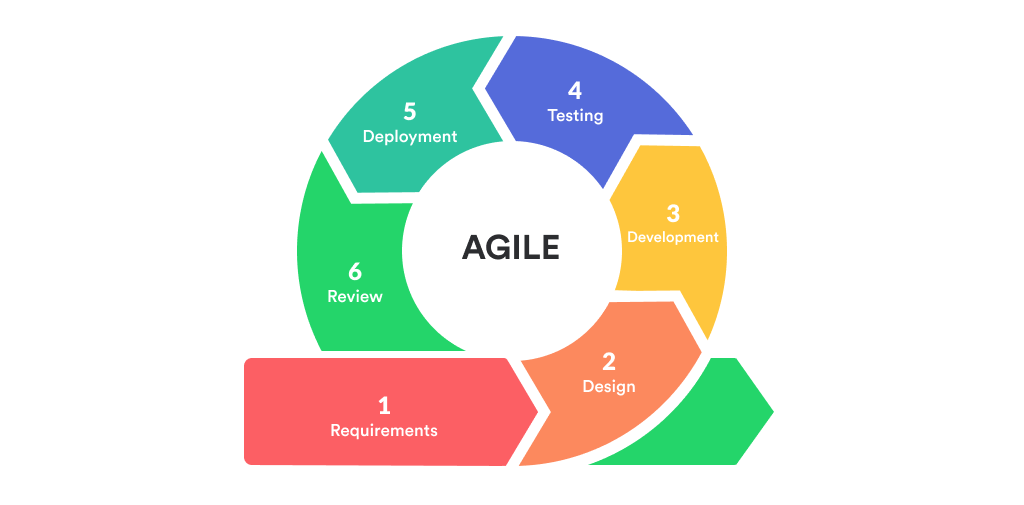
\includegraphics[width=0.9\textwidth]{images/agile.png}
\end{figure}	

The popularity of Agile development methodologies among the software development industry has increased since their introduction in the mid-nineties \cite{AGILE_SURVEY}, with almost 86\% of surveyed international software developers using agile methodologies in their work \cite{AGILE_SURVEY_TWO}.

\subsection{Comparing Agile and Waterfall}
Following supervisory and team meetings, research and analysis, both Agile and Waterfall were compared under the following headings:

\begin{description}
  \item[$\bullet$] Applicability and Compatibility with the Project
  \item[$\bullet$] Requirement Delivery
  \item[$\bullet$] Flexibility
\end{description}

With the establishment of the aforementioned headings, comparisons were drawn between both approaches.

\begin{table}[H]
\begin{tabularx}{\linewidth}{>{\parskip1ex}X@{\kern4\tabcolsep}>{\parskip1ex}X}
\toprule
\hfil\bfseries Agile
&
\hfil\bfseries Waterfall
\\\cmidrule(r{3\tabcolsep}){1-1}\cmidrule(l{-\tabcolsep}){2-2}

%% PROS, seperated by empty line or \par
\begin{compactitem}[-]
\item[+] Strong ability to respond to the changing project requirements.
\item[+] Issues and roadblocks can be detected and addressed rapidly. 
\item[+] Feedback is immediate and helps drive development.
\item[+] Attractive methodologies that would fit the nature and goal of the project, namely \textbf{Kanban} and  \textbf{Scrum}.
\item[+] Encourages frequent end-user involvement, considering college students would be the target audience for the application this Agile benefit is especially attractive. 
\item[$-$] Lack of emphasis on necessary designing and documentation.
\item[$-$] Project may grow ever-larger since there isn't a clearly defined end point.

\end{compactitem}
\par

&

%% CONS, seperated by empty line or \par
\begin{compactitem}[-]
\item[+] Clearly defined and formalized requirements.
\item[+] The software development structure is carefully planned and detailed, minimizing the number of potential issues and roadblocks.
\item[+] Progress is easily measured, the beginning and end points for each phase are fixed allowing easier progress tracking.
\item[$-$] Analysis, planning and requirements definition phase can end up taking time out of actually developing the project.
\item[$-$] Low flexibility level meaning it may be difficult if not impossible to make major changes to the project while in the middle of development, considering the ever changing nature of the defined application this would be troublesome.
\end{compactitem}

\\\bottomrule
\end{tabularx}
\caption{Comparisons drawn between Agile \& Waterfall}
\end{table}

Following comparisons being drawn it became clear to the team an \textbf{Agile} approach would best suit the outlined project. This approach would enable many benefits but those that were the most attractive to bring to the project included:

\begin{enumerate}
  \item \textbf{Interactive user involvement and feedback} - Having the target audience of the application be students while still being in college surrounded by potential users meant this was hugely beneficial.
  \item \textbf{The ability to develop via small periodic releases} - Based on feedback from supervisors and other students the priorities may shift and sway, small incremental changes mean there would be increased flexibility and versatility when it came to adapting to change.
  \item \textbf{Kanban and Scrum Methodologies} - The idea of incremental releases combined with periodic sprints based on workflow defined via the Kanban method was something that the team agreed would improve the overall flow of development following supervisory discussions.
\end{enumerate}

\section{Agile Approach}
Given the ever changing requirements and nature of the project and for additional reasons outlined in the analysis section, the integration of Agile methodologies would be crucial to ensure an effective development cycle.

\paragraph{}
Deciding what Agile methodologies to incorporate into the project was the next step, Kanban and Scrum were two that had already been identified and deemed highly beneficial. Following more research into methodologies including Extreme Programming (XP) and Feature Driven Development (FDD) TODO THE REST OF THIS AT A LATER DATE**

\subsection{Kanban}
Since development began the Kanban methodology was adhered to. The Kanban method is essentially a lean method to manage and improve flow systems. Like Scrum, Kanban is a process intended to help teams work together more effectively and efficiently \cite{KANBAN_SCRUM}. 

\paragraph{}
Kanban allows a team to easily prioritize and visualize the main elements of the project in-progress and also easily delegate tasks based on what work needs to be started, what work is in progress and what has been completed.

\begin{figure}[H]
	\caption{Github Kanban}
	\label{image:kanban}
	\centering
	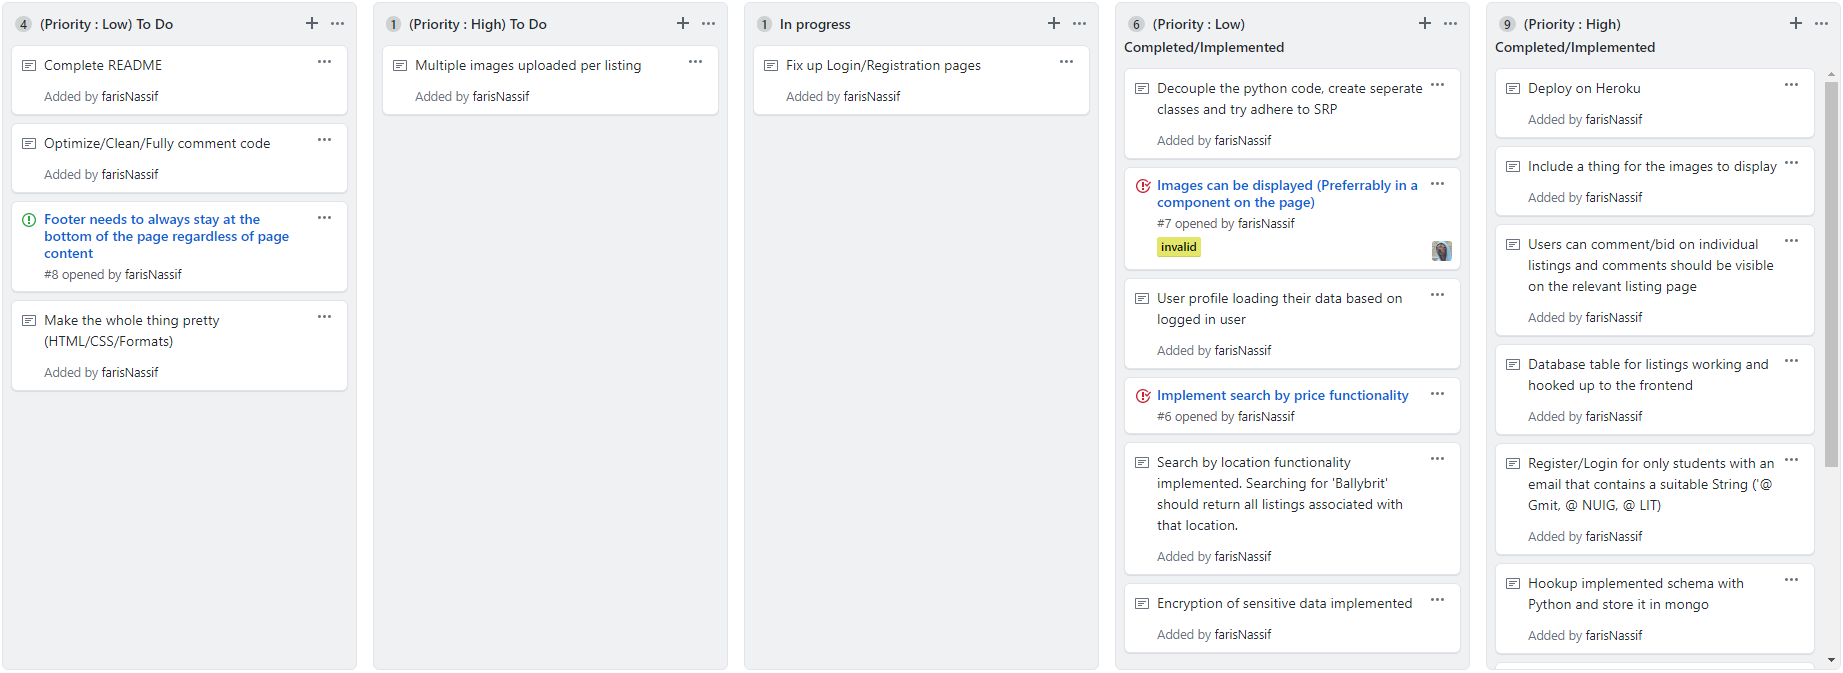
\includegraphics[width=1\textwidth]{images/kanban.png}
\end{figure}

Figure \ref{image:kanban} above consists of the Kanban board used during the development of the project. The Kanban board consists of four main columns:

\begin{enumerate}
  \item \textbf{To Do - Low Priority}
  \item \textbf{To Do - High Priority}
  \item \textbf{In Progress}
  \item \textbf{Completed}
\end{enumerate}

Initially the team had planned to use Trello \cite{TRELLO} for project tracking, however following discussions with other students and finally supervisory discussions it was found that Github had a built in Kanban function. 

\paragraph{}
Having the ability to track the progress of the project on the same platform as where the project is actually being collaborated on would be a huge benefit, it meant issues and commits could be assigned to  tasks listed on the Kanban board meaning team members could work with more efficiency than if an external tracker like Trello was used.

\subsection{Scrum}
In addition to Kanban, the Scrum methodology was incorporated and employed. The Scrum methodology is very efficient when paired with the Kanban methodology. Sprints were employed and carried out by the team. A Sprint is a time-limited iteration of the continuous development cycle \cite{SCRUM}. Sprints were generally one week in length. At the end of each week, a supervisory meeting would be conducted where the team would communicate their progress throughout the week and also any issues or blockers were brought to the attention of the supervisor.

\paragraph{}
At the end of the meeting, goals for the next Sprint were defined and potential solutions and avenues of exploration were discussed. Any new goal was included on the Kanban board and assigned to a team member. Based on previous information gathering, these tasks were undertaken in the determined priority order.

\section{Version Control}
Initially Github \cite{GITHUB} was the only platform considered for version control coverage, however following discussions with other students, Gitlab \cite{GITLAB} was spoken highly of, so this was another potential consideration. 

\paragraph{}
Github had the home advantage of being a platform that had been used extensively by the team in previous projects, however Gitlab isn't too different and is likely only less popular since it's a newer platform. Both platforms are git based software-development platforms that provide access control and several collaboration features for developers. 

\paragraph{}
The main advantage of GitLab for the team was its open source nature, which allows the hosting of your repositories on your own server free of charge. Gitlab's continuous integration pipelines were also very attractive, Github requires the employment of third-party tools tools like Travis-CI to avail of features like this.

\paragraph{}
The advantages of Gitlab were nice, however following internal discussions it was decided Github would remain the main source of Version Control for the project. The main reason for this being the advantages of Gitlab wouldn't be able to be as utilized as the team would like. Github being familiar and not too different from Gitlab meant there wasn't any deal-breaker that would merit the switch.

\subsection{Github}
A Github repository was setup remotely and used during development to allow for collaboration, code security and to track the progress of the project as well as providing the functionality of managing dependencies and providing alerts if new versions should arise. 

\paragraph{}
The team took advantage of many of the additional features Github has to offer including it's Kanban board, the ability to branch and merge was utilized but could have been used more and the option to open and assign issues to name a few.